\documentclass[sigconf,review,anonymous]{article}
% if you need to pass options to natbib, use, e.g.:
%     \PassOptionsToPackage{numbers, compress}{natbib}
% before loading neurips_2020

% ready for submission
%\usepackage{neurips_2020}

% to compile a preprint version, e.g., for submission to arXiv, add add the
% [preprint] option:
%     \usepackage[preprint]{neurips_2020}

% to compile a camera-ready version, add the [final] option, e.g.:
     \usepackage[final]{neurips_2020}

% to avoid loading the natbib package, add option nonatbib:
     %\usepackage[nonatbib]{neurips_2020}
\usepackage{multirow}
\usepackage[table,xcdraw]{xcolor}
\usepackage[utf8]{inputenc} % allow utf-8 input
\usepackage[T1]{fontenc}    % use 8-bit T1 fonts
% \usepackage{hyperref}       % hyperlinks
% \usepackage{url}            % simple URL typesetting
\usepackage{booktabs}       % professional-quality tables
\usepackage{amsfonts}       % blackboard math symbols
\usepackage{nicefrac}       % compact symbols for 1/2, etc.
\usepackage{microtype}      % microtypography
\usepackage{float} % here for H placement parameter
% \usepackage{multirow}
% \usepackage[normalem]{ulem}
% \useunder{\uline}{\ul}{}
% \usepackage{xcolor}
\usepackage[table,xcdraw]{xcolor}
\usepackage[obeyspaces]{url}
\usepackage{graphicx}
\usepackage{listings}
\usepackage{enumerate}
\definecolor{codegreen}{rgb}{0,0.6,0}
\definecolor{codegray}{rgb}{0.5,0.5,0.5}
\definecolor{codepurple}{rgb}{0.58,0,0.82}
\definecolor{backcolour}{rgb}{0.95,0.95,0.92}



\lstset{style=mystyle}
\usepackage{algorithm}
\usepackage[noend]{algpseudocode}

\makeatletter
% Reinsert missing \algbackskip
\def\algbackskip{\hskip-\ALG@thistlm}
\makeatother


\title{Realizing Literate Programming using Neural Machine Translation}

% The \author macro works with any number of authors. There are two commands
% used to separate the names and addresses of multiple authors: \And and \AND.
%
% Using \And between authors leaves it to LaTeX to determine where to break the
% lines. Using \AND forces a line break at that point. So, if LaTeX puts 3 of 4
% authors names on the first line, and the last on the second line, try using
% \AND instead of \And before the third author name.
\author{%
  Anonymous Author(s)
}
% \author{%
  
%   Hung Phan \\
%   Department of Computer Science \\
%   Iowa State University\\
%   Ames, IA 50011 \\
%   hungphd@iastate.edu \\
% }

\begin{document}

\maketitle

\begin{abstract}
Literate Programming (LP) is a programming paradigm that unites natural language with code as one document, which helps the developer to explain the logic of some parts of the code both ways of representation. However, despite having advantages for code understanding,  LP hasn't been popularly applied in practice for two reasons. First, developers are required to specify the code for each natural language description manually which is a tedious and error-prone process. Secondly, supervised machine learning approaches for automatically retrieving code from Natural Language is expensive since it required a big dataset of the parallel corpus with NL and Programming Language. In this paper, we provide a tool InvocMap to realize LP to allow developers for writing the textual description of Method Invocations (MIs) inside code environment and get the correct MIs. Different from other code suggestion tools as AnyCode which was only considered natural language as input, we analyze the input from 2 sources: the NL description and its surrounding context. InvocMap proposes a semi-supervised approach by 3 modules. First, it uses unsupervised Neural Embedding to handle NL description of MIs to a list of possible method names. Second, Machine Translation models are trained from large scale code corpus to learn the structure of MIs given a list of method names and surrounding code context. Third, a program analysis step is proposed to assign local variables to structure of MIs to get the final code. InvocMap provides 2 modes of input for describing MIs for developers: from method names directly and from natural language description. By evaluation with training data from 1000 Java high-quality projects, we got the accuracy as up to 90\% for MI suggestion from method names and over 60\% for MI suggestion from NL description, which is outperforming the prior work AnyCode and showing the potential of realizing LP which is specified for supporting NL descriptions of MIs.
\end{abstract}

\section{Introduction}
Literate Programming (LP), which was invented by Donald E. Knuth \cite{001}, is intended to support software developers by a convenient programming environment. The idea of LP is to construct a sample program by an alternative way. The construction of program by LP is considered as a process contained two observations. First, they can consider the program as a list of statements which is handled by a compiler in programming language. This observation is traditional and be familiar with developers. The second observation is to consider a programming task as a description in the form of natural language. Unlike the first observation, the second observation proposes a new way of program representation by literature. It helps the program not only runnable but also explanable in human natural language. An application of LP is the WEB system \cite{001}, which can output the program as natural description and programming language in Pascal by Tangle and Waive library. LP does not only provide advantages in better programming experiences, but also introduce a solution for education of how to programming, based on the appearance of documentation for each code snippets.
\\
Despite having many advantages, the LP program paradigm has not been used popularly since its appearance in 1984. Based on our knowledge, the most recent application which applied LP is provided by  Haghish et al \cite{005}, which provide support for visualizing LP in HTML format. The most well-known LP dataset is \cite{006}, which provides LP dataset of code which are in the form of combination between Natural Language (NL) and code. \cite{004} studies about the problems which 
prevent LP to be practical. First, the number of developers who can be good at programming and documenting their code are limited. In the other words, developers seems to be good only at the first observation than the second observation of LP. Secondly, all of LP system like \cite{006} require manually defining the source code related to each natural language description. The cost for manually representing the code by NL and programming language (PL) for every code snippets of large scale corpus is expensive. Thus, it is important to have a system that automatically deriving the code from NL description in a code environment, to make LP feasible.
\\
From our knowledge, there is no tools or research projects which work directly on generating code for natural language parts for support LP in Software Engineering (SE) and Machine Learning (ML). However, the problem of generating code from natural language (NL) is one of interesting research problem in SE. In these works, AnyCode \cite{007} provides a solution for synthesizing expression, mostly in the form of Method Invocations (MIs) by proposing the language model called Probabilistic Context Free Grammar (PCFG). Other works applied and optimized Machine Translation (MT) by providing supervised approaches for inferring code from natural description and vice versa. \cite{008} provides a tree based code generation which can be integrated in Recurrent Neural Network (RNN) for Python. \cite{009} applied Statistical Machine Translation (SMT) model for learning pseudo code from actual code for code summarixation. This trend of research require manually annotated data for supervised learning, which is expensive when applied in other types of NL. Although NL description and code can be extracted from large scale code repository, parallel corpus extracted by this way is usually erroneous and contain noise.  Barone  et al. \cite{010} conduct a Python corpus by automatically extracting documentation and implementation of the same Python methods. By the experiment, they show that applying Machine Translation models to this corpus is challenging since the accuracy on both SMT and Neural Machine Translation (NMT) are low.
\\
All of current works on generating code from natural language input like \cite{007,008,009,010} were not designed to support LP. They treat the natural language as the entire input and provide the output as generated code, without considering the information from surrounding code. \cite{010} considered the input as natural description of functions in Java Documentation (JavaDoc) for each functions of Python. AnyCode (\cite{007}) provides a solution for getting MIs by NL queries instead of NL element inside the code. In the other words, the output of expressions generated from AnyCode is consistent regardless the surrounding code.
\\
In this paper, we want to realizing Literate Programming by providing InvocMap, a tool that helps developers to define natural language description of method invocations at any locations inside the code environment and automatically suggesting MIs for all descriptions. Unlike prior works, we consider the input as a LP code snippet, which considers code as the combination of sequence of code elements and natural language elements (NL-E). We provide the output as code snippet that all of NL-E were transformed to MIs. To achieve the solution, we provide a semi-supervised approach which combines three techniques: neural embedding to get method names from surrounding context and natural language element; machine translation to get the parsed tree of MIs; Program Analysis to analyze the surrounding context to instrument information to tree to get the final code. We provide following contributions:
\begin{itemize}
	\item Provided another viewpoint for considering natural language element with information of code before and after it. 
	\item Implemented an approach for automatically generating possible method names based on all NL and code information. 
	\item Built a Machine Translation model which converted from text to tree data structure of Method Invocation.
	\item Provided a code suggestion tool InvocMap to realizing LP by 2 modes. In the first mode, we allow developers to input method names and other information to get the method invocations. In the second mode, developers can write free form NL elements and get suggested code as list of MIs which the highest ranking suggested option as the most relevant code suggested by InvocMap.
\end{itemize}

\section{Background}
In this part, we provide description for important terms we use for this research. Besides terms are wellknown in Software Engineering, we define a set of terms which are mentioned as elements in our approach.

\begin{enumerate}[\indent {}]
        \item \textbf{Abstract Syntax Tree (AST)} is a tree representation of tokens which are generated from statements and expressions in programming language (PL) (\cite{011}).
        \item \textbf{Method Invocation (MI)} is one type of AST. MI can be described by combination of 2 elements: the parsed tree and local variables/ literals which are usually located at the leaf level of the tree \cite{012}. 
        \item \textbf{Structured AST (S-AST)} is the data structure that we defined in this paper. S-AST is the tree representation of MI but doesn't include information about name of local variables/ literals. S-ASTs are extracted by visiting MIs in code corpus and abstracting local variables. An example of S-AST is shown in Figure \ref{figMotivatingExample}.
        \item \textbf{Core Method Name (C-MN)} is the name of MI which is appeared as the root node of S-AST. For example, in Figure \ref{figMotivatingExample}, the C-MN is \texttt{containsKey}. 
        \item \textbf{Literate Programming Code Snippet (LP-CS)} is a code snippet that contains one to multiple natural language description (element) for method invocations. LP-CS contains 3 below elements.
        \item \textbf{Natural Language Element (NL-E), PreCode and PostCode}: NL-E is the description in NL. \textbf{PreCode} of NL-E is the list of code tokens appeared before NL-E. \textbf{PostCode} is the list of code tokens appeared after NL-E. Example of NL-E is shown in Figure \ref{figMotivatingExample}.
        
        \item \textbf{Variables and Terms of NL-E}: Variables of NL-E are all tokens related to string and numeric literal along with variables defined in NL-E. Terms of NL-E are tokens of NL-E which are not in list of variables. 
        
        
        
        
    \end{enumerate}




\section{The \textit{InvocMap} Model}
\subsection{Problem Formulation}
\begin{figure}
   
        \center{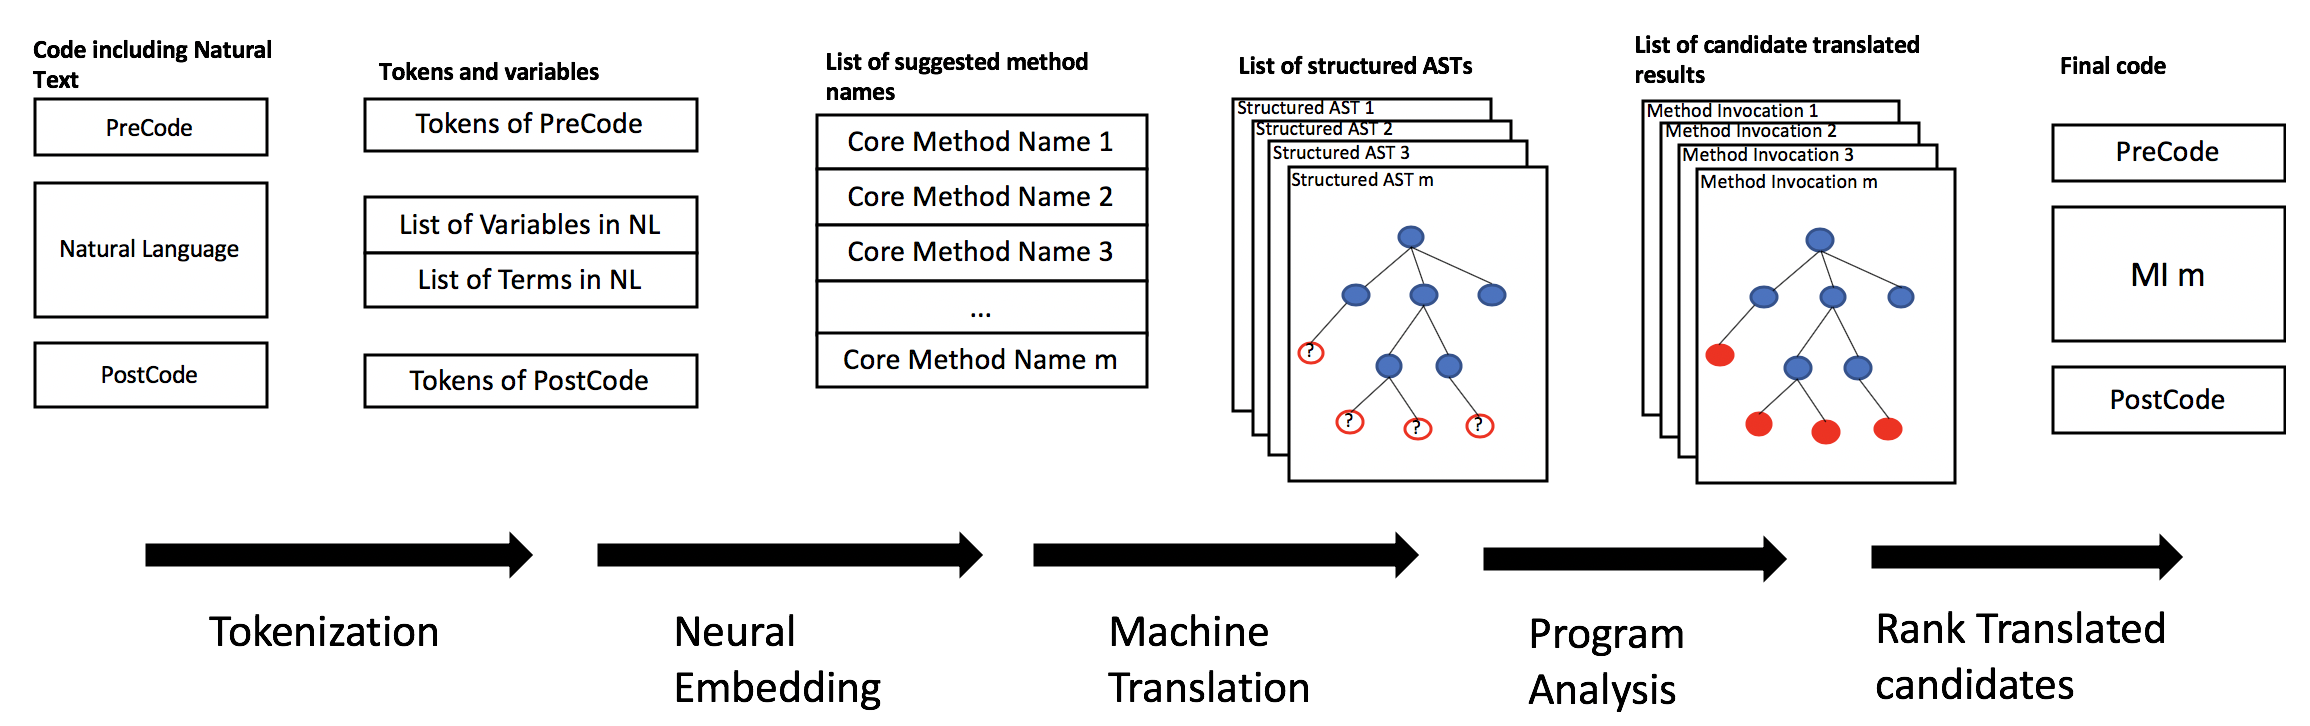
\includegraphics[width=\linewidth]
        {images/InvocMapOverview.png}}
        \caption{Overview of InvocMap model}
        \label{figOverview} 
\end{figure}
\begin{figure}
        \center{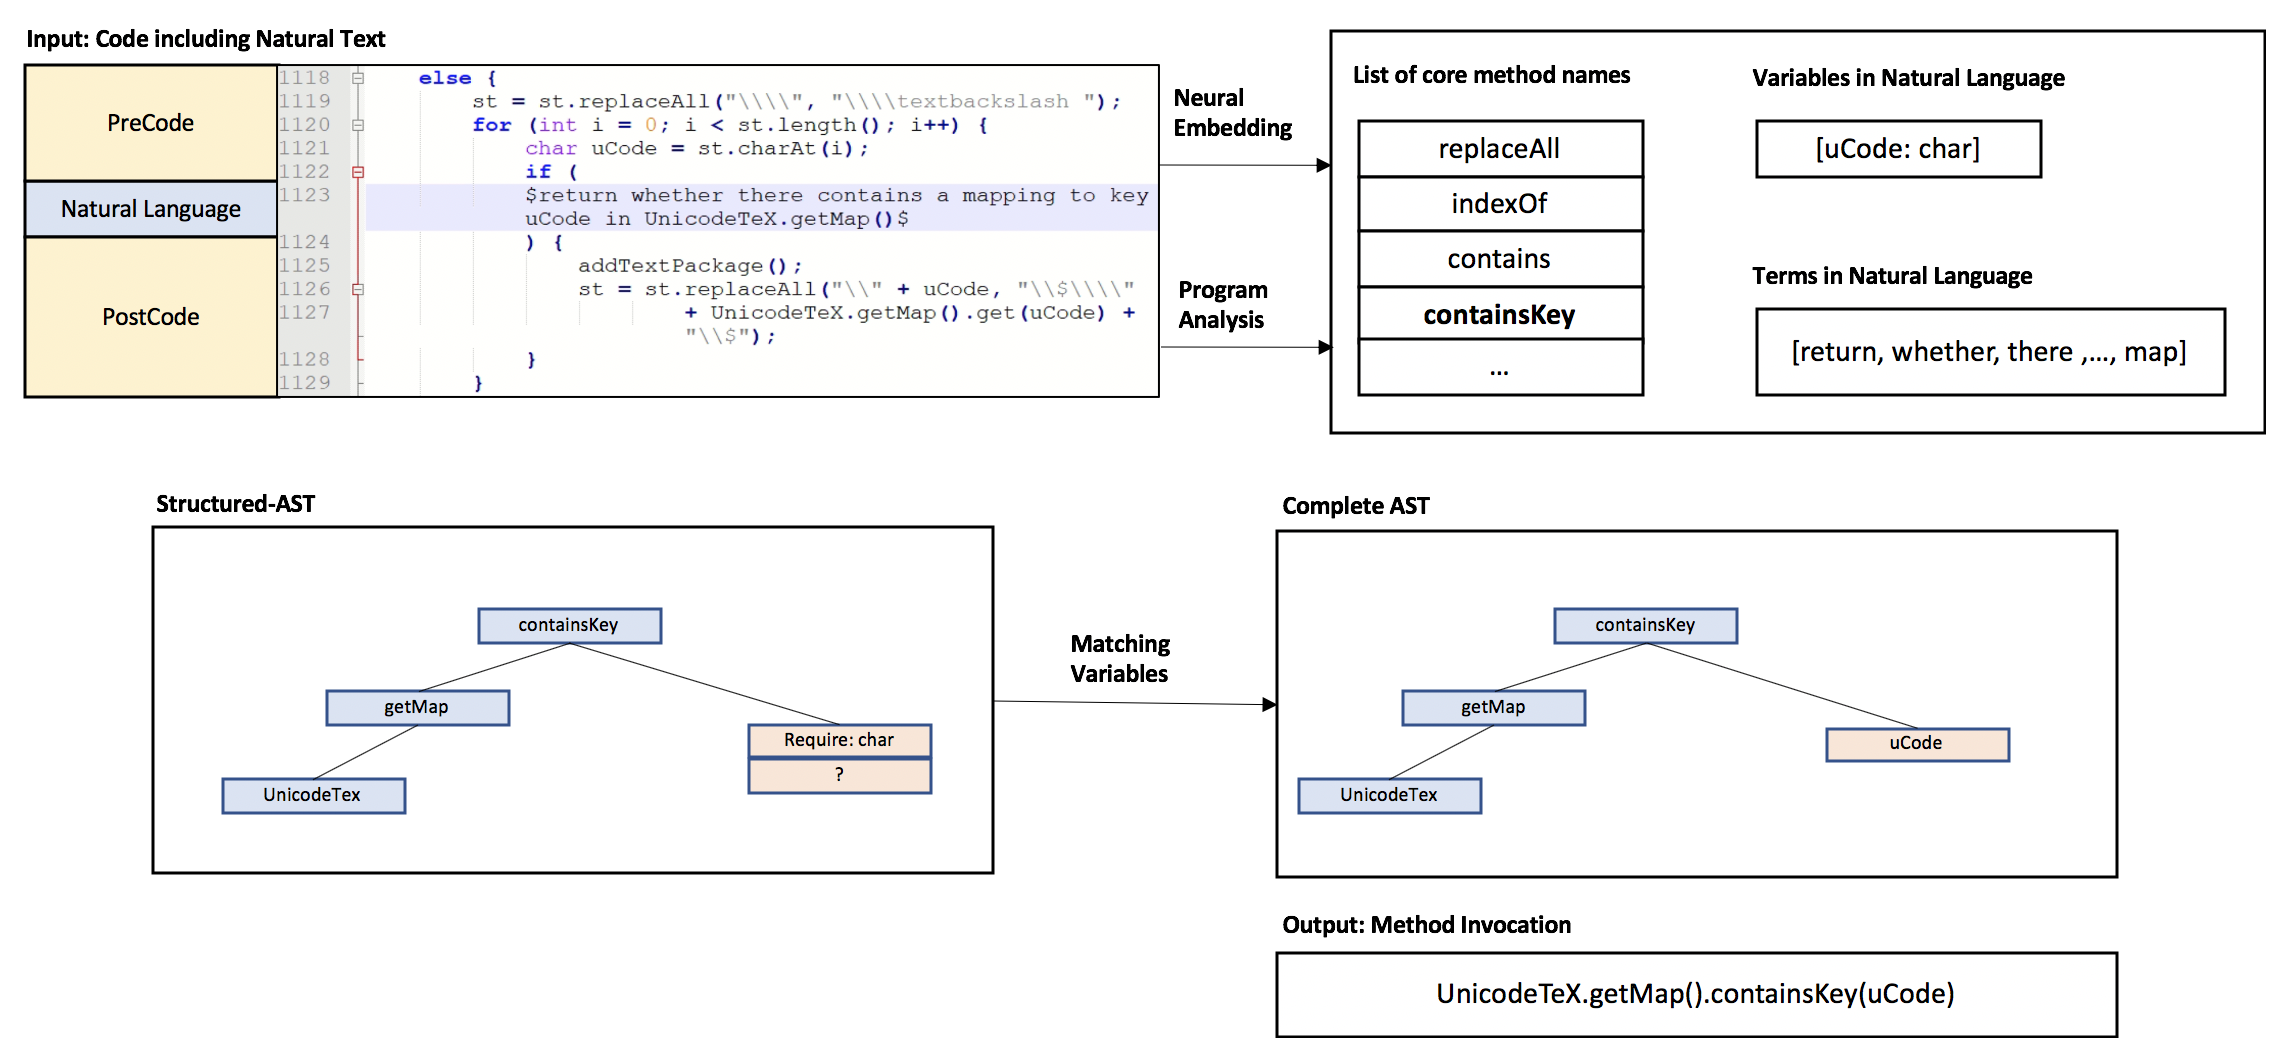
\includegraphics[width=\linewidth]
        {images/MotivatingExample.png}}
        \caption{Motivating Example of InvocMap}
        \label{figMotivatingExample} 
\end{figure}
\subsection{Code and Natural Language tokenization}
\subsection{Neural Embedding based for core method name inference}
% \begin{LTXexample}[style=ListingSample,caption={Algorithm for C-MN inference from NL element},label={algmNeuralEmbedding}]
% \begin{lstlisting}[language=Octave,caption={Algorithm for C-MN inference from NL element},label={algmNeuralEmbedding}]  
% Input:
%     Literate Programming Code C;
%     List of method contexts in training set M[];
%     Size of list of suggested method names k;
% Output: 
%     List of method names O;

% %prepare models by training data
% preModel <- trainDoc2VecByPreCodeTokens(M)
% postModel <- trainDoc2VecByPostCodeTokens(M)

% %get list of suggested method names from precode and postcode
% preMethods <-getClosestMethods(C,preModel,k)
% postMethods <-getClosestMethods(C,postModel,k)

% %combine 2 list of suggestions
% O <-combineAndFilter(preMethods,postMethods)


% \end{lstlisting}

\begin{algorithm}
    \caption{Algorithm for C-MN inference from NL element}\label{algmNeuralEmbedding}
    \hspace*{\algorithmicindent} \textbf{Input:}
     Literate Programming Code C;
    List of method contexts in training set M[];
    Size of list of suggested method names k;
    \\
    \hspace*{\algorithmicindent} \textbf{Output:} 
    List of method names O;
    \begin{algorithmic}[1]
    \Procedure{getSuggestedMethodNamesFromNaturalInput}{}
%    \Procedure{MyProcedure}{$x,y$}
%     % Input:
%     \Comment{Input: x}
%     % Output:
%     \Comment{Output:y}

    \State $\textit{preModel} \gets \textit{trainDoc2VecByPreCodeTokens(M)} $
    \Comment{prepare models by training data}
    \State $\textit{postModel} \gets \textit{trainDoc2VecByPostCodeTokens(M)} $
    \\
    \State $\textit{preMethods} \gets \textit{getClosestMethods(C,preModel,k)} $
    \Comment{get list of suggested method names}
    \State $\textit{postMethods} \gets \textit{getClosestMethods(C,postModel,k)} $
    \\
    \State $\textit{O} \gets \textit{combineAndFilter(preMethods,postMethods)} $
    \Comment{combine 2 lists of suggestions}
    
    \EndProcedure
    \end{algorithmic}
    \end{algorithm}
\subsection{Structured AST generation}
\subsection{Assigning variables to Structured AST}
\subsection{Ranking translated candidates }
\section{Evaluation}
\subsection{Data Preparation}
\begin{table}[]
\centering
\begin{tabular}{|l|r|}
\hline
\multicolumn{1}{|c|}{\textbf{Item}}                & \multicolumn{1}{c|}{\textbf{Number}} \\ \hline
Java projects                                      & 1000                                 \\ \hline
Size of Neural Embedding (NE) corpus               & 1770000                              \\ \hline
Size of Machine Translation corpus                 & 800000                               \\ \hline
Size of extrinsic corpus for NE                    & 120                                  \\ \hline
Size of extrinsic corpus for NL to code evaluation & 100                                  \\ \hline
Number of developers conduct in study of Q1        & 2                                    \\ \hline
Number of code snippet with NL in Q1               & 40                                   \\ \hline
\end{tabular}
\end{table}
\subsection{Baseline Method}
\subsection{Q1. How developers need for code suggestion from Method Name and from Natural Language}

\begin{table}[]
\centering
\begin{tabular}{|l|r|r|r|}
\hline
\multicolumn{1}{|c|}{\textbf{Input}} & \multicolumn{1}{l|}{\textbf{Cannot}} & \multicolumn{1}{l|}{\textbf{SomeParts}} & \multicolumn{1}{l|}{\textbf{AllParts}} \\ \hline
Core Method Name                     & 10\%                                 & 35\%                                    & 55\%                                   \\ \hline
Natural Language                     & 40\%                                 & 20\%                                    & 40\%                                   \\ \hline
\end{tabular}
\end{table}

\subsection{Q2. Accuracy of Neural Embedding for suggesting core method names  from natural language and surrounding code}

\begin{table}[]
\centering
\begin{tabular}{|l|l|l|l|}
\hline
\textbf{} & \textbf{PreCode}          & \textbf{PostCode}         & \textbf{Combine}          \\ \hline
Acccuracy & \multicolumn{1}{r|}{76\%} & \multicolumn{1}{r|}{76\%} & \multicolumn{1}{r|}{93\%} \\ \hline
\end{tabular}
\end{table}

\subsection{Q3. Accuracy of Machine Translation models for inferring structured AST from core method names}

\begin{table}[]
\centering
\begin{tabular}{|l|r|r|r|r|r|r|}
\hline
\multicolumn{1}{|c|}{\textbf{Types of Evaluation}} & \multicolumn{3}{c|}{\textbf{Cross Validation}}                                                                    & \multicolumn{3}{c|}{\textbf{Extrinsic evaluation}}                                                                \\ \hline
\multicolumn{1}{|c|}{\textbf{Metric}}              & \multicolumn{1}{c|}{\textbf{Precision}} & \multicolumn{1}{c|}{\textbf{Recall}} & \multicolumn{1}{c|}{\textbf{F1}} & \multicolumn{1}{c|}{\textbf{Precision}} & \multicolumn{1}{c|}{\textbf{Recall}} & \multicolumn{1}{c|}{\textbf{F1}} \\ \hline
Core Method Name (C-MN)                            & 70.43                                   & 75.89                                & 73.06                            & 62.54                                   & 75.8                                 & 68.53                            \\ \hline
C-MN and variables                                 & 84.04                                   & 78.98                                & 81.43                            & 86.01                                   & 81.16                                & 83.51                            \\ \hline
C-MN, variables and terms                          & 89.33                                   & 79.98                                & 84.4                             & 86.88                                   & 81.31                                & 84                               \\ \hline
\end{tabular}
\end{table}

\subsection{Q4. Accuracy of InvocMap model for inferring code for realizing Literate Programming}

\begin{table}[]
\centering
\begin{tabular}{|l|r|}
\hline
\multicolumn{1}{|c|}{\textbf{Approach}} & \multicolumn{1}{c|}{\textbf{Accuracy in Top 1}} \\ \hline
AnyCode                                 & 44\%                                            \\ \hline
InvocMap                                & 61.19\%                                         \\ \hline
\end{tabular}
\end{table}

\begin{table}[]
\centering
\begin{tabular}{|l|r|}
\hline
\multicolumn{1}{|c|}{\textbf{Top result}} & \multicolumn{1}{c|}{\textbf{Accuracy}} \\ \hline
Top-1                                     & 61.19\%                                \\ \hline
Top-2                                     & 64.94\%                                \\ \hline
Top-3                                     & 68.13\%                                \\ \hline
Top-4                                     & 69.04\%                                \\ \hline
Top-5                                     & 70.02\%                                \\ \hline
\end{tabular}
\end{table}

\begin{table}[]
\centering
\begin{tabular}{|l|r|}
\hline
\multicolumn{1}{|c|}{\textbf{Top result}} & \multicolumn{1}{c|}{\textbf{Num of exact-match}} \\ \hline
InvocMap Top-1                            & 31                                               \\ \hline
InvocMap Top-10                           & 37                                               \\ \hline
\end{tabular}
\end{table}

\begin{table}[]
\centering
\begin{tabular}{|l|l|}
\hline
\multicolumn{1}{|c|}{\textbf{ID}} & \multicolumn{1}{c|}{\textbf{Natural Language / Expected result / Translated result}}        \\ \hline
\multicolumn{1}{|r|}{33}          & return square root of minDelta for Math                                                     \\ \hline
\rowcolor[HTML]{DAE8FC} 
                                  & \cellcolor[HTML]{DAE8FC}                                                                    \\ \cline{1-1}
\rowcolor[HTML]{DAE8FC} 
                                  & \multirow{-2}{*}{\cellcolor[HTML]{DAE8FC}Math.sqrt(minDelta)}                               \\ \hline
\multicolumn{1}{|r|}{44}          & attempt to establish connection to given jdbcUrl DbUser DbPwd for DriverManager             \\ \hline
\rowcolor[HTML]{DAE8FC} 
                                  & \cellcolor[HTML]{DAE8FC}                                                                    \\ \cline{1-1}
\rowcolor[HTML]{DAE8FC} 
                                  & \multirow{-2}{*}{\cellcolor[HTML]{DAE8FC}DriverManager.getConnection(jdbcUrl,DbUser,DbPwd)} \\ \hline
\multicolumn{1}{|r|}{2}           & return whether there contains a mapping to key uCode in UnicodeTeX.getMap()                 \\ \hline
\rowcolor[HTML]{DAE8FC} 
                                  & \cellcolor[HTML]{DAE8FC}                                                                    \\ \cline{1-1}
\rowcolor[HTML]{DAE8FC} 
                                  & \multirow{-2}{*}{\cellcolor[HTML]{DAE8FC}UnicodeTeX.getMap().containsKey(uCode)}            \\ \hline
\multicolumn{1}{|r|}{80}          & return the minimum of lp.height and height                                                  \\ \hline
\rowcolor[HTML]{FFCCC9} 
                                  & Math.min(lp.height,height)                                                                  \\ \hline
\rowcolor[HTML]{FFCCC9} 
                                  & Math.min(height,lp.height)                                                                  \\ \hline
\multicolumn{1}{|r|}{20}          & format now.getTime() into String and append to dateFormatter for SimpleDateFormat           \\ \hline
\rowcolor[HTML]{FFCCC9} 
                                  & dateFormatter.format(now.getTime())                                                         \\ \hline
\rowcolor[HTML]{FFCCC9} 
                                  & dateFormatter.format(now.getTime()).toString()                                              \\ \hline
\multicolumn{1}{|r|}{68}          & return a color from default key "MenuItem.acceleratorForeground" for UIManager              \\ \hline
\rowcolor[HTML]{FFCCC9} 
                                  & UIManager.getColor("MenuItem.acceleratorForeground")                                        \\ \hline
\rowcolor[HTML]{FFCCC9} 
                                  & UIManager.put("MenuItem.acceleratorForeground",color)                                       \\ \hline
\end{tabular}
\end{table}

\section{Related Work}
\section{Conclusion and Future Work}

\clearpage
\bibliography{references}{}
%this may not be right style for nips
\bibliographystyle{plain}


\end{document}
